\chapter{Osciladores senoidales.}\label{osc}


\hspace{10pt} En los sistemas electrónicos surge con frecuencia la necesidad de
contar con señales periódicas que tengan una forma de onda
estándar,por ejemplo, ondas senoidales, cuadradas, triangulares,
pulsadas, etc.

En este capítulo se estudian únicamente los métodos más frecuentes
para obtener ondas senoidales. En particular el método que utiliza
el concepto de realimentación y consiste en un amplificador y una
red selectiva en frecuencia R-C o L-C. La amplitud de las ondas
generadas se limita , o ajusta, por medio de mecanismos no lineales.
No obstante lo dicho anteriormente, se conocen a este tipo de
circuitos que generan ondas senoidales a través de fenómenos de
resonancia, como \textbf{osciladores lineales}.

\section{Principios básicos}

\hspace{10pt} En este punto se estudian los principios básicos de los
\textbf{osciladores lineales}, como se mencionó anteriormente se
tiene que emplear alguna forma de no linealidad para obtener el
control de la amplitud de la onda de salida. De hecho todos los
osciladores son, estrictamente hablando, circuitos no lineales.

Para poder utilizar las herramientas de análisis y diseño de
sistemas lineales se procede en dos pasos: primero se considera al
sistema idealmente lineal, utilizando los criterios circuitales y de
realimentación conocidos; y luego se hace uso de mecanismos no
lineal para controlar la amplitud. Este método, si bien no es
exacto, es útil en la práctica y está amplia y eficientemente
probado. En cualquier caso podrían utilizarse herramientas para el
cálculo no lineal del sistema si se necesitara mayor precisión.


\subsection{Osciladores senoidales como sistemas realimentados}

\hspace{10pt} En el capítulo 2 se trató el tema de la estabilidad de los sistemas
realimentados, específicamente en la figura \ref{estab1} se muestra
que la ubicación de los polos sobre el eje imaginario indicaba que
el sistema iba a presentar oscilaciones sostenidas. Este es el
concepto fundamental a aplicarse en los osciladores senoidales, es
decir se utilizan sistemas realimentados que, al menos idealmente,
posean polos en el eje imaginario, de modo que puedan sostener
oscilaciones aún sin una excitación de entrada.

En la figura \ref{estab2} se muestra un sistema realimentado. En el
caso de osciladores consideraremos que la entrada es nula ($x_i=0$)
y además, como se explicó en el capítulo 2, el límite de estabilidad
está en: $1+T(s)=1+a(s)f(s)=0$.

En el caso de osciladores se modificará, por simplicidad, la figura
\ref{estab2}. La figura \ref{osc1} muestra el mismo sistema que la
figura \ref{estab2} con las siguientes consideraciones: $x_i=0$
(entrada nula), la red a(s) se denomina red amplificadora, la red
f(s) se la renombra como $\beta(s)$ y se la denomina red atenuadora
selectiva en frecuencia y se elimina el elemento restador. Bajo
estas circunstancias es fácil deducir que el límite de estabilidad
pasa a ser: $a(s)\beta(s)=1$.

El esquema de la figura \ref{osc1} es el que se utiliza generalmente
para osciladores senoidales, es decir una etapa amplificadora y un
red selectiva en frecuencia en la red de ralimentación.

\begin{figure}
	\centering
	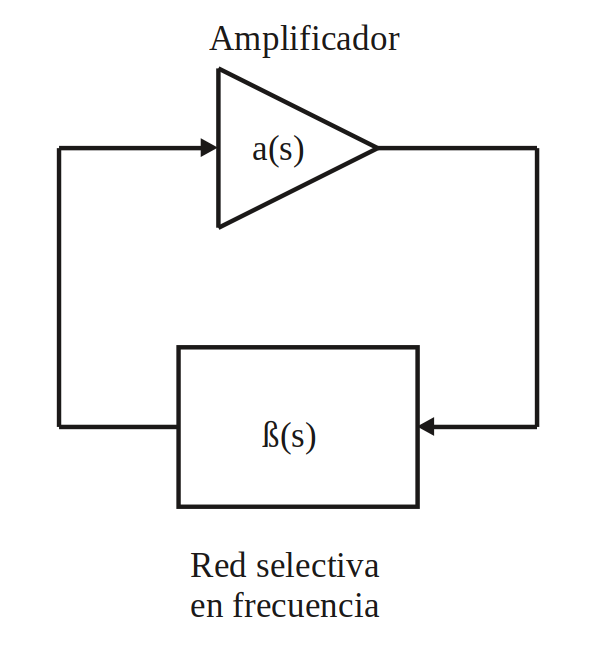
\includegraphics[width=2.5in]{figuras/osc1.png}\\
	\caption{Esquema teórico de un oscilador senoidal.}\label{osc1}
\end{figure}

\subsection{Criterio de oscilación}

\hspace{10pt} Si a una frecuencia angular específica $w_o$ la ganancia de lazo
$a(w_o)\beta(w_o)=1$ el sistema será un oscilador, es decir tendrá
una salida finita sin excitación en su entrada. Para que el sistema
oscile senoidalmente a la frecuencia $w_o$ la condición antedicha
sólo debe cumplirse a una frecuencia ($w_o$). Esto se conoce como
criterio de oscilación de \textbf{Barkhausen}.

El criterio de Barkhausen puede desdoblarse en:


\begin{eqnarray}
	\nonumber
	|a(w_o)\beta(w_o)|&=& 1 \quad a)\\
	\nonumber
	\Phi[a(w_o)\beta(w_o)]&=& 0 \quad b)\\
	\nonumber
\end{eqnarray}

La expresión a) es la denominada condición de amplitud. En la
práctica la red $\beta$ es una red selectiva en frecuencia, siendo
$w_o$ su frecuencia central de mínima atenuación. A dicha frecuencia
la amplificación $a(w_o)$ será igual la inversa de la atenuación de
la red selectiva en frecuencia ($1/\beta(w_o)$), de modo que la
ganancia de lazo total sea uno.

La expresión b) es la condición de fase, que establece que el
desfasaje de la ganancia de lazo debe ser nulo a la frecuencia
$w_o$.

En los sistemas que se abordan la frecuencia de oscilación $w_o$
está determinada sólo por la fase de la ganancia de lazo $\Phi[a
\beta(w)]$. Siendo esta frecuencia la que cumple la condición de
fase del criterio de Barkhausen.

En la figura \ref{osc2} a) se muestra en forma esquemática la curva
de fase en función de la frecuencia de un determinado oscilador. La
curva de trazo lleno representa el pasaje por $0°$ de dicho
oscilador, mientras que la de trazo discontinuo muestra la misma
situación ante cambios en los parámetros del sistema. Se ve allí que
la frecuencia de oscilación ha variado en $\Delta w$ para una
variación de fase $\Delta \Phi$. En la figura \ref{osc2} b) se
muestra la curva de fase de otro oscilador con una pendiente menor.
En ella se evidencia que para una variación $\Delta\Phi$ igual al
caso anterior la variación de frecuencia $\Delta w$ es mayor. Se
muestra, intuitivamente, que cuanto mayor sea la pendiente de la
curva de fase, en su pasaje por $0°$, los osciladores tendrán una
variación menor en su frecuencia de oscilación con respecto a
variaciones en sus parámetros, es decir serán más estables en
frecuencia. Todas estas cuestiones tiene en cuenta, por supuesto,
que en todo momento se cumpla la condición de amplitud.


\begin{figure}
	\centering
	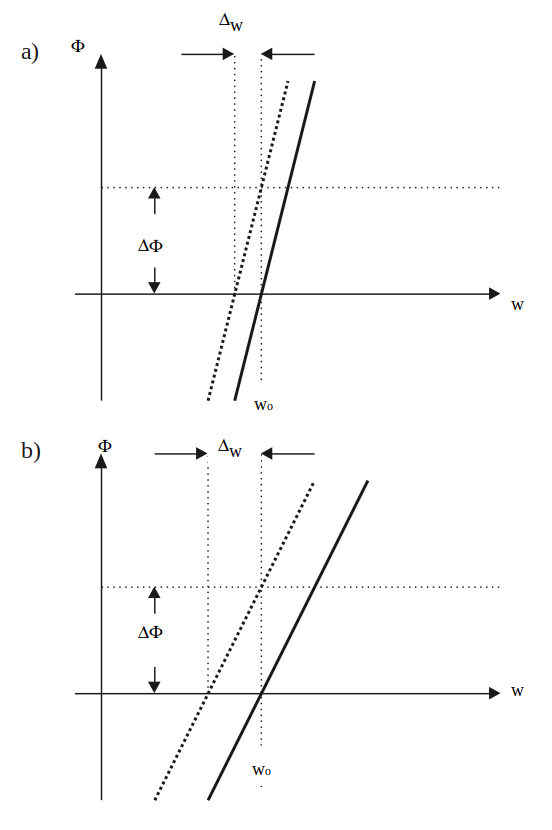
\includegraphics[width=3.5in]{figuras/osc2.png}\\
	\caption{Curva de fase de la ganancia de lazo de dos osciladores genéricos.}\label{osc2}
\end{figure}

La estabilidad en frecuencia es una característica de gran
importancia en el diseño de osciladores. Una manera de cuantificarla
es calculando el Factor de Estabilidad en Frecuencia (SF), este
cuantificador relativo se define como:
\begin{equation*}
	SF=w_o \left| \frac{\displaystyle \delta \Phi}{\displaystyle \delta w} \right|_{w=w_o}
\end{equation*}

Los osciladores diseñados mediante una red atenuadora muy selectiva
en frecuencia, y por lo tanto con una curva de fase muy abrupta,
tendrán una gran estabilidad en frecuencia.

\subsection{Control no lineal de amplitud}

\hspace{10pt} El criterio de oscilación de Barkhausen garantiza oscilaciones
senoidales en un sentido matemático. Si por medio de ajustes
lográramos que el sistema cumpla exactamente la condición
$a\beta(w_o)=1$, es sabido que esta situación sería imposible de
mantenerla en el tiempo, ya que variaciones inevitables de los
parámetros (por ejemplo por temperatura) harían que los polos
imaginarios puros se desplazaran a uno u otro lado en el plano s. Si
los polos se desplazaran hacia la izquierda del eje imaginario (zona
estable) las oscilaciones cesarían. Por el contrario, si los polos
se movieran hacia el semiplano derecho, la amplitud de las
oscilaciones tendería a aumentar siendo limitadas por la saturación
de los dispositivos activos, generando señales oscilantes con alto
grado de distorsión. Es sabido, además, que la amplitud de la señal
de salida de un sistema con polos en el eje imaginario dependerá en
forma teórica de las condiciones iniciales.

Estos dos efectos, la variación de los parámetros y la dependencia
de la amplitud de salida de las condiciones iniciales, hacen
necesario un mecanismo de control no lineal de la ganancia del
sistema.

Básicamente el mecanismo de control debe cumplir con lo siguiente:
\begin{itemize}
	\item En primera instancia se debe diseñar el sistema para que los polos
	se encuentren en la mitad derecha del plano s,  con la precaución de
	que estén cercanos al eje imaginario. Esta condición se obtiene
	modificando el criterio de Barkhausen de modo que se cumpla la
	condición de fase $\Phi[a(w_o)\beta(w_o)]= 0$ y que se cumpla en
	exceso la condición de amplitud $|a(w_o)\beta(w_o)|> 1$,  de esta
	manera aseguramos que los polos iniciales estén en el semiplano
	derecho. Para que no haya excesiva distorsión en la señal
	de salida la condición de amplitud debe diseñarse para que se cumpla
	en exceso pero en menos de un 10 \%, como criterio práctico.
	\item En el caso del ítem anterior, si se conecta la fuente de
	alimentación, la amplitud de las oscilaciones tiende a
	incrementarse, cuando la amplitud llega a un nivel deseado, la
	red no lineal entra en acción y hace que la ganancia de lazo se
	reduzca exactamente a la unidad. En otras palabras los polos
	serán "movidos" al eje jw. Esto hará que el circuito sostenga
	oscilaciones a la amplitud deseada, si por algún motivo la
	ganancia de lazo se redujera por debajo de la unidad, la
	amplitud tenderá a disminuir, esto será detectado por la red no
	lineal, que hará que la ganancia de lazo aumente lo necesario
	para llegar nuevamente a la unidad.
\end{itemize}

Hay dos métodos básicos para el control no lineal de la amplitud. El
primer método se basa en un amplificador lineal por tramos cuya
transferencia genérica se muestra en la figura \ref{osc3}, en la
zona de ganancia \textbf{$a_1$} la condición de amplitud se cumple
en exceso y en las zonas de ganancia \textbf{$a_2$} se cumple en
defecto, este tipo de amplificadores puede diseñarse con un circuito
similar al mostrado en la figura \ref{ao32}. Si se diseña para que
las diferencias entre las pendientes sean "suaves" se puede lograr
un control en la amplitud con una reducida distorsión no lineal en
la señal de salida. Esta distorsión puede ser reducida también por
la acción del filtro de la red selectiva en frecuencia del lazo de
realimentación.

El otro mecanismo para control de amplitud se basa en la utilización
de dispositivos que presenten resistencia variable controlada por el
nivel de amplitud de la señal de salida. Estos dispositivos, puestos
de modo que afecten en la ganancia de lazo, harán disminuir o
aumentar dicha ganancia en función de lo requerido, variando en
forma apropiada su resistencia. Por ejemplo se pueden utilizar
transistores de efecto de campo, no en su zona de saturación, sino
en su zona de conductancia variable en función de su tension
gate-source.

\begin{figure}
	\centering
	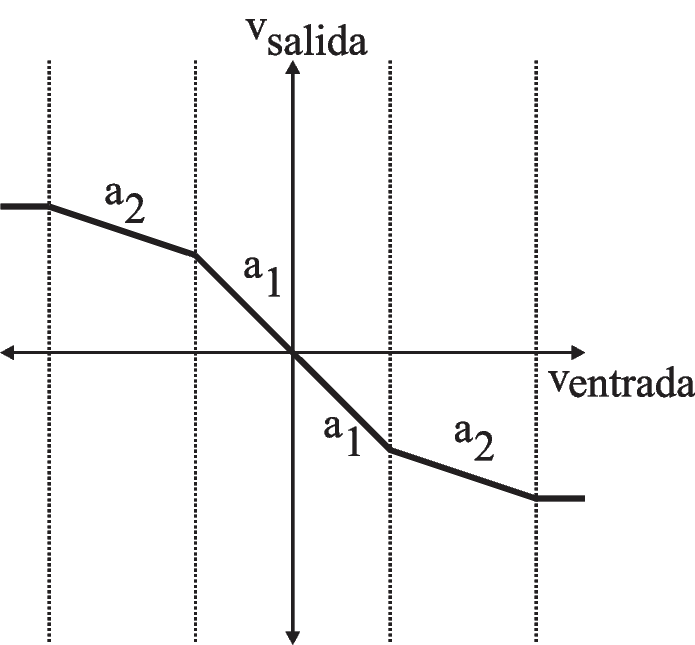
\includegraphics[width=3.5in]{figuras/osc3.png}\\
	\caption{Amplificador lineal por tramos genérico.}\label{osc3}
\end{figure}


\section{Circuitos osciladores R-C}

\hspace{10pt} A continuación se detallan algunos de los circuitos osciladores que utilizan dispositivos
activos y redes RC.

\subsection{Oscilador puente de Wien}

\hspace{10pt} Este circuito es uno de los osciladores de diseño más sencillo y está basado
en el puente de Wien. En la figura \ref{osc4} a) se muestra el esquema
circuital de este tipo de osciladores sin tener en cuenta la red no
lineal de control de amplitud. En dicha figura se muestra que el
circuito está formado por un amplificador operacional conectado en
su configuración no inversora, con una ganancia determinada por las
resistencias $R_1$ y $R_2$ cuyo valor es de $1+\frac{\displaystyle R_2}{\displaystyle R_1}$ y
por una red de realimentación selectiva en frecuencia formada por
las resistencias $R_A$ y $R_B$ y por los capacitores $C_A$ y $C_B$.
Para obtener la expresión de la ganancia de lazo se busca un punto
apropiado para abrirlo, en este circuito el punto apropiado es el
marcado como ``x'' en la figura \ref{osc4} a) ya que presenta impedancia elevada. Al abrir el lazo en
dicho punto se calcula la ganancia de lazo por medio del circuito
mostrado en la figura \ref{osc4} b), que es un equivalente del caso
a) abierto en el punto ``x'' y cargado convenientemente en el punto
de apertura (en este caso cargado con una impedancia infinita). La
ganancia de lazo obtenida de esta forma es la siguiente:


\begin{eqnarray}\label{ecuosc1}
	\nonumber
	a\beta(jw)&=&\frac{\displaystyle v_{x'}}{\displaystyle v_x}=\frac{\displaystyle v_{x'}}{\displaystyle v_a}\frac{\displaystyle v_a}{\displaystyle v_x}=\frac{\frac{\displaystyle R_B}{\displaystyle 1+jwC_BR_B}}{\frac{\displaystyle R_B}{\displaystyle 1+jwC_BR_B}+R_A+\frac{\displaystyle 1}{\displaystyle
			jwC_A}}\left(1+\frac{\displaystyle R_2}{\displaystyle R_1}\right)\\
	\nonumber
	&=&\frac{\displaystyle jwC_AR_B\left(1+\frac{\displaystyle R_2}{\displaystyle R_1}\right)}{1-w^2C_AC_BR_AR_B+jw\left(C_AR_B+C_AR_A+C_BR_B\right)}\\
\end{eqnarray}

Como ya se enunció, de la condición de fase se obtiene la frecuencia
$w_o$ a la cual la ganancia de lazo tiene desfasaje $0°$, de la
expresión \ref{ecuosc1} se ve que el desfasaje $0°$ se obtiene
cuando $1-w^2C_AC_BR_AR_B=0$, es decir que la frecuencia de
oscilación será:
\begin{equation*}
	w_o=\frac{\displaystyle 1}{\displaystyle \sqrt{C_AC_BR_AR_B}}
\end{equation*}

De la condición de amplitud (en $w=w_o$) se obtiene la condición de
ganancia necesaria para que el sistema oscile. De la expresión
\ref{ecuosc1} se obtiene:
\begin{eqnarray}
	\nonumber
	\frac{\displaystyle \left(1+\frac{\displaystyle R_2}{\displaystyle R_1}\right)C_AR_B}{\displaystyle C_AR_B+C_AR_A+C_BR_B}&>&1\\
	\nonumber
	\left(1+\frac{\displaystyle R_2}{\displaystyle R_1}\right)&>&1+\frac{\displaystyle R_A}{\displaystyle R_B}+\frac{\displaystyle C_B}{\displaystyle C_A}\\
	\nonumber
\end{eqnarray}

Si se diseña $R_A=R_B=R$ y $C_A=C_B=C$ la frecuencia de oscilación
será $w_0=\frac{\displaystyle 1}{\displaystyle RC}$ y la ganancia
necesaria para que el sistema oscile deberá ser
$\left(1+\frac{\displaystyle R_2}{\displaystyle R_1}\right)>3$, es
decir para que se inicien las oscilaciones $R_2$ deberá ser
ligeramente mayor que $2R_1$.

Para controlar adecuadamente la amplitud puede utilizarse un
circuito de ganancia lineal por tramos, como el mostrado en la
figura \ref{osc5}.

\begin{figure}
	\centering
	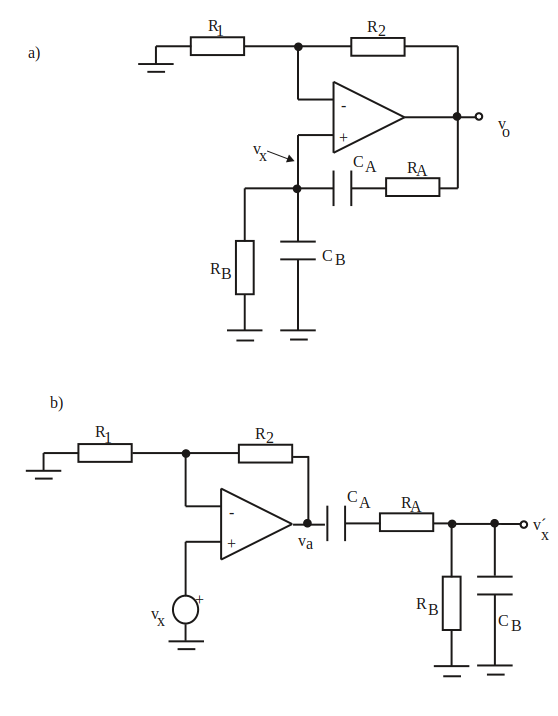
\includegraphics[width=4in]{figuras/osc4.png}\\
	\caption{Oscilador puente de Wien. a) Esquema circuital básico, b) circuito para el cálculo de la ganancia de lazo.}\label{osc4}
\end{figure}

\begin{figure}
	\centering
	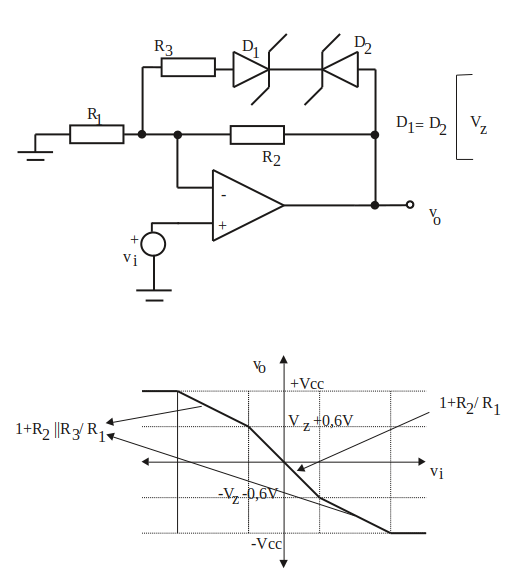
\includegraphics[width=4in]{figuras/osc5.png}\\
	\caption{Amplificador con ganancia lineal por tramos.}\label{osc5}
\end{figure}

\subsection{Oscilador de desplazamiento de fase}

\hspace{10pt} La estructura básica de un oscilador de desplazamiento de fase es la
mostrada en la figura \ref{osc6} a), en ella se ve un amplificador
de tensión de ganancia $-K$ y una red en escalera de (al menos) tres
etapas R-C. El amplificador tiene un desplazamiento de fase de
$180°$, por lo tanto la red de realimentación R-C deberá desplazar
otros $180°$ a la frecuencia de oscilación para que se cumpla la
condición de fase. Además la atenuación de la red de realimentación
a la frecuencia de oscilación debe ser $1/K$ para que se cumpla la
condición de amplitud. Esta configuración es la denominada de atraso
de fase, si se invierten las posiciones entre los capacitores y los
resistores de la red el oscilador se denomina de adelanto de fase.

En la figura \ref{osc6} b) se ve el circuito luego de abrir el lazo
en el punto ``x'', se supone que el amplificador tiene una
impedancia de entrada $\rightarrow \infty$, por lo que al abrir el
lazo en dicho punto no afecta el cálculo de la transferencia de
lazo.

De la figura \ref{osc6} b) se derivan las siguientes expresiones:

\begin{eqnarray}\label{ecuosc2}
	\nonumber
	-Kv_x&=&i_1\left(R_o+R+\frac{\displaystyle 1}{jwc}\right)-i_2R\\
	\nonumber
	0&=&-i_1R+i_2\left(R+aR+\frac{\displaystyle a}{jwc}\right)-i_3aR\\
	\nonumber
	0&=&-i_2aR+i_3\left(aR+a^2R+\frac{\displaystyle a^2}{jwc}\right)\\
	\nonumber
	v_x'&=&i_3a^2R\\
\end{eqnarray}

De las expresiones \ref{ecuosc2} se halla la ganancia de lazo
$\frac{\displaystyle v_x'}{\displaystyle v_x}(jw)$. Si en esta
transferencia se anula la parte imaginaria, se obtiene la frecuencia
de oscilación (condición de fase), la expresión es:
\begin{equation}\label{ecuosc3}
	w_{o}=\frac{\displaystyle 1}{\displaystyle RC}\frac{\displaystyle 1}{\displaystyle \sqrt{3+\frac{\displaystyle 2}{\displaystyle a}+\frac{\displaystyle 1}{\displaystyle a^2}+\frac{\displaystyle R_o}{\displaystyle R}\left(\frac{\displaystyle 2}{\displaystyle a}+2\right)}}
\end{equation}

Si se cumple que a la frecuencia $w_o$ la transferencia
$\frac{\displaystyle v_x'}{\displaystyle v_x}(jw_o)>1$ (condición de
amplitud), el circuito oscilará. De esta condición se obtiene que:

\begin{equation}\label{ecuosc4}
	K>8+\frac{\displaystyle 12}{\displaystyle a}+\frac{\displaystyle 7}{\displaystyle a^2}+\frac{\displaystyle 2}{\displaystyle a^3}+\frac{\displaystyle R_o}{\displaystyle
		R}\left(8+\frac{\displaystyle 11}{\displaystyle a}+\frac{\displaystyle 4}{\displaystyle a^2}\right)+\left(\frac{\displaystyle R_o}{\displaystyle
		R}\right)^2\left[2+\frac{\displaystyle 2}{\displaystyle
		a}\right]
\end{equation}

\begin{figure}
	\centering
	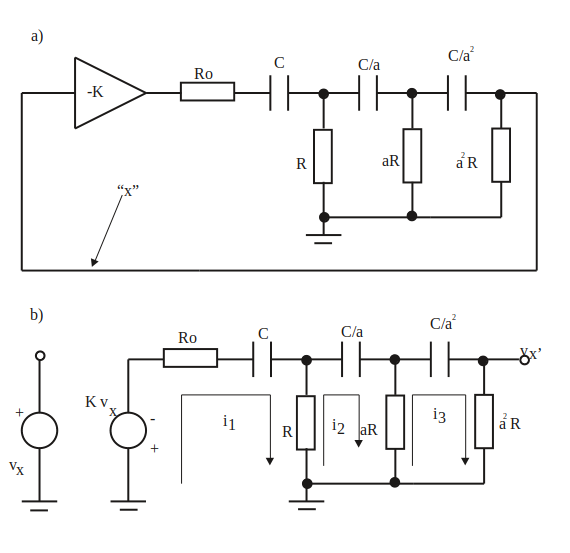
\includegraphics[width=4in]{figuras/osc6.png}\\
	\caption{Oscilador de desplazamiento de fase. a) Esquema circuital básico. b) Circuito para el cálculo de las condiciones de oscilación.}\label{osc6}
\end{figure}

En la figura \ref{osc7} a) se muestra un circuito práctico. El
transistor bipolar, en configuración emisor común, da la
amplificación y el desplazamiento de fase necesarios; mientras que
la red R-C proporciona la atenuación y la selectividad adecuada para
que a la frecuencia $w_o$ se cumplan las condiciones de oscilación.
Si se abre el lazo en la base del transistor el circuito equivalente
será el mostrado en la figura \ref{osc7} b). En este caso en
particular el parámetro "a" del circuito de la figura \ref{osc6}
se hace igual a uno; además la resistencia $R_x$ debe ser tal que
$R_x\parallel R_1\parallel R_2\parallel h_{ie}=R$ de modo que, con el
efecto de carga incluido, el punto $v_x'$ presente efectivamente una impedancia de valor equivalente a $R$.
Haciendo un equivalente de Thèvenin en el colector del transistor se
ve  que la ganancia $K$ de la figura \ref{osc6} es
$K=\frac{h_{fe}R_o}{h_{ie}}$. La resistencia de emisor, desacoplada
a la frecuencia $w_o$, puede ser utilizada para ajustar la
polarización del transistor y por lo tanto ajustar la ganancia del
mismo para llevarlo a condiciones de oscilación. De la figura
\ref{osc7} b) y de las ecuaciones \ref{ecuosc3} y \ref{ecuosc4} se
obtiene la frecuencia de oscilación $f_{osc}$ y la transconductancia
del transistor necesaria $g_m=\frac{h_{fe}}{h_{ie}}$:

\begin{eqnarray}\label{ecuosc5}
	\nonumber
	f_{osc}&=&\frac{\displaystyle 1}{\displaystyle 2 \pi R C} \frac{\displaystyle 1}{\displaystyle \sqrt{6+4\frac{\displaystyle R_o}{\displaystyle R}}}\\
	\nonumber
	g_mR_o&>&29+23\frac{\displaystyle R_o}{\displaystyle R}+4\left(\frac{\displaystyle R_o}{\displaystyle R}\right)^2\\
\end{eqnarray}

\begin{figure}
	\centering
	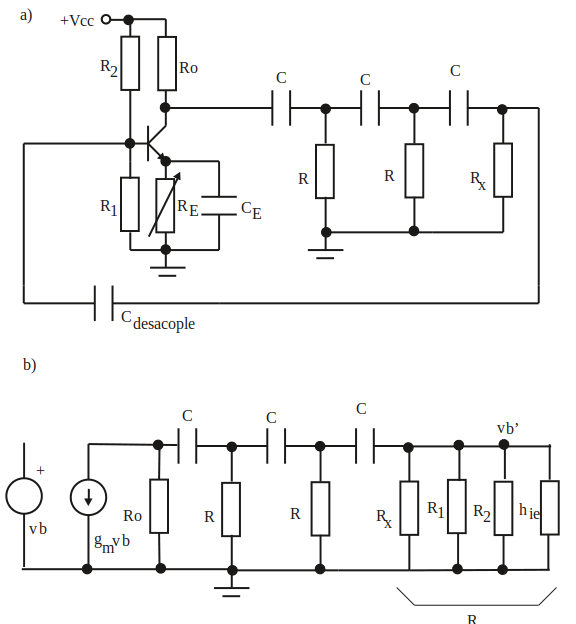
\includegraphics[width=4in]{figuras/osc7.png}\\
	\caption{Ejemplo de oscilador de desplazamiento de fase práctico. a) Esquema circuital. b) Circuito para el cálculo de las condiciones de oscilación.}\label{osc7}
\end{figure}


\section{Osciladores L-C y a cristal}

\subsection{Familia de osciladores L-C}

\hspace{10pt} En la figura \ref{osc8} se muestra el esquema circuital básico de
los osciladores L-C. El amplificador desplaza la fase $180°$ y la
red de realimentación está compuesta por una red $\Pi$ con
reactancias puras.

\begin{figure}
	\centering
	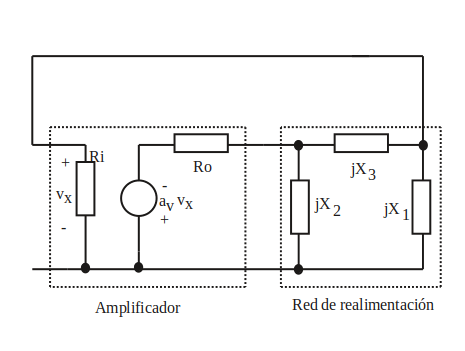
\includegraphics[width=4in]{figuras/osc8.png}\\
	\caption{Esquema circuital básico de los osciladores L-C.}\label{osc8}
\end{figure}

Las características principales de este tipo de osciladores son:

\begin{itemize}
	\item Se utilizan a frecuencias superiores que los osciladores
	R-C ya vistos.
	\item La gran selectividad propia de los circuitos L-C de alto
	factor de calidad $Q$, hacen que las señales generadas a la
	salida de la red de realimentación sean senoidales con bajo
	nivel de distorsión.
	\item Buena estabilidad en frecuencia. Se puede demostrar que
	ésta depende directamente del Q del circuito sintonizado.
\end{itemize}

En el estudio de estos osciladores se utilizará, en primera
instancia, un modelo sencillo de los dispositivos activos que no
incluyan los efectos de alta frecuencia. Luego se podrán extrapolar
los resultados incorporándolos adecuadamente. Los elementos pasivos
se considerarán ideales.

En definitiva se trata de utilizar modelos simples que deriven
formulas de sencilla interpretación y utilización. En los ejemplos
desarrollados se utilizarán elementos de ajuste (inductores,
capacitores o resistores variables) que inevitablemente deberán
existir en un diseño real.

En la figura \ref{osc9} a) se muestra el esquema que se utiliza para
el desarrollo general de este tipo de osciladores. Estando
constituido el amplificador por un dispositivo activo del tipo de un
transistor bipolar o de efecto de campo. En el punto ``x'' se abre
el lazo, en la figura \ref{osc9} b) se muestra el circuito para
calcular las condiciones de oscilación con el efecto de carga
correspondiente.

\begin{figure}
	\centering
	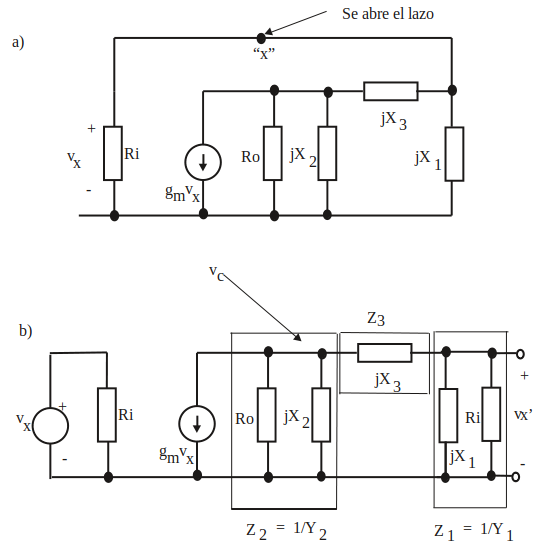
\includegraphics[width=4in]{figuras/osc9.png}\\
	\caption{Osciladores L-C: a) esquema general con transistores, b) circuito para el cálculo de las condiciones de oscilación. }\label{osc9}
\end{figure}

De la figura \ref{osc9} b) las ecuaciones nodales que se derivan
son:

\begin{eqnarray}\label{ecuosc6}
	\nonumber
	v_cY_2+g_mv_x+\frac{\displaystyle v_c-v_x'}{\displaystyle Z_3}&=&0\\
	\nonumber
	v_x'Y_1+\frac{\displaystyle v_x'-v_c}{\displaystyle Z_3}&=&0\\
\end{eqnarray}
De las ecuaciones \ref{ecuosc6} y de la condición de Barkhausen se obtiene:

\begin{equation}\label{ecuosc7}
	\frac{\displaystyle v_x'}{\displaystyle v_x}(w_o)=\frac{\displaystyle -g_m}{\displaystyle
		Y_1+Y_2+Y_1Y_2Z_3}=1 + j0
\end{equation}

Si se cumplen las siguientes condiciones:

\begin{eqnarray}
	\nonumber
	R_i \gg \mid X_1\mid_{w_o}\quad\Rightarrow Y_1=\frac{\displaystyle 1}{\displaystyle jX_1}\\
	\nonumber
	Z_3=jX_3\\
	\nonumber
	Y_2=\frac{\displaystyle 1}{\displaystyle R_o}+\frac{\displaystyle 1}{\displaystyle jX_2}
	\nonumber
\end{eqnarray}

Y se reemplaza en la ecuación \ref{ecuosc7}, se obtiene:

\begin{equation}\label{ecuosc8}
	\frac{\displaystyle v_{x'}}{\displaystyle v_x}(w_o)=-\frac{\displaystyle g_m}{\displaystyle \frac{\displaystyle 1}{\displaystyle R_o}+\frac{\displaystyle X_3}{\displaystyle R_oX_1}+\frac{\displaystyle 1}{\displaystyle j}\left(\frac{\displaystyle 1}{\displaystyle X_1}+\frac{\displaystyle 1}{\displaystyle X_2}+\frac{\displaystyle X_3}{\displaystyle
			X_1X_2}\right)}=1+j0
\end{equation}

Si se anula la parte imaginaria de la ecuación \ref{ecuosc8} se
obtiene la condición de fase:

\begin{equation}\label{ecuosc9}
	X_1+X_2+X_3=0
\end{equation}

Cumpliéndose la condición de fase, $X_1+X_3=-X_2$, se deriva de la
ecuación \ref{ecuosc8} la condición de amplitud:

\begin{equation}\label{ecuosc10}
	g_mR_o=\frac{\displaystyle X_2}{\displaystyle X_1}
\end{equation}

Por lo tanto la condición de arranque será:

\begin{equation}\label{ecuosc11}
	g_mR_o>\frac{\displaystyle X_2}{\displaystyle X_1}
\end{equation}

De la condición de amplitud se deduce que el signo de la reactancia
$X_1$ tiene que ser el mismo que el signo de la reactancia $X_2$; de
lo anterior dicho y de la condición de fase se obtiene que el signo
de la reactancia $X_3$ tiene que ser el opuesto del signo de las
otras dos.

Por lo tanto surgen dos posibilidades sencillas mostradas en la
figura \ref{osc10}. En el caso a) la red de realimentación está
formada por dos capacitores y un inductor, y se denomina oscilador
Colpitts; mientras que en el caso b) la red está formada por dos
inductores y un capacitor denominándose oscilador Hartley.

En el caso de la figura \ref{osc10} a) la condición de fase de la
ecuación \ref{ecuosc9} será:

\begin{equation}\label{ecuosc12}
	-\frac{\displaystyle 1}{\displaystyle w_oC_2}-\frac{\displaystyle 1}{\displaystyle
		w_oC_1}+w_oL_3=0
\end{equation}

De aquí se obtiene la frecuencia de oscilación:

\begin{equation}\label{ecuosc13}
	w_o=\frac{\displaystyle 1}{\displaystyle \sqrt{L_3\frac{C_1C_2}{C_1+C_2}}}
\end{equation}

La condición de arranque será (derivada de la ecuación
\ref{ecuosc11}):

\begin{equation}\label{ecuosc14}
	g_mR_o>\frac{\displaystyle X_2}{\displaystyle X_1}=\frac{\displaystyle C_1}{\displaystyle C_2}
\end{equation}

De la figura \ref{osc10} b) y de la condición de fase se obtiene,
suponiendo que no existe inductancia mutua entre $L_1$ y $L_2$, lo
siguiente:

\begin{equation}\label{ecuosc15}
	-\frac{\displaystyle 1}{\displaystyle w_oC_3}+w_oL_1+w_oL_2=0
\end{equation}

\begin{equation}\label{ecuosc16}
	w_o=\frac{\displaystyle 1}{\displaystyle \sqrt{(L_1+L_2)C_3}}
\end{equation}

De la condición de arranque:

\begin{equation}\label{ecuosc17}
	g_mR_o>\frac{\displaystyle X_2}{\displaystyle X_1}=\frac{\displaystyle L_2}{\displaystyle L_1}
\end{equation}

En caso que existiera inductancia mutua entre $L_1$ y $L_2$, las
expresiones anteriores serían:

\begin{equation}\label{ecuosc18}
	w_o=\frac{\displaystyle 1}{\displaystyle \sqrt{(L_1+L_2+2M)C_3}}
\end{equation}


\begin{equation}\label{ecuosc19}
	g_mR_o>\frac{\displaystyle X_2}{\displaystyle X_1}=\frac{\displaystyle L_2+M}{\displaystyle L_1+M}
\end{equation}

\begin{figure}
	\centering
	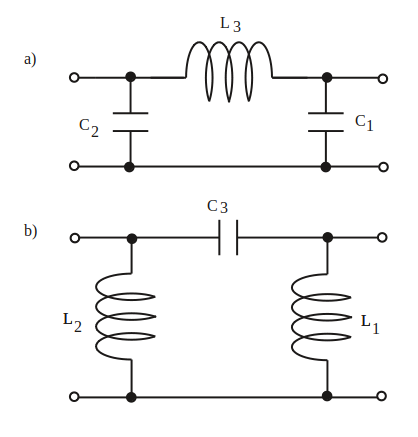
\includegraphics[width=3in]{figuras/osc10.png}\\
	\caption{Red de realimentación de osciladores L-C: a) Colpitts, b) Hartley. }\label{osc10}
\end{figure}

Una variante del Colpitts es la configuración Clapp mostrada en la
figura \ref{osc11}. En ella se ve que el inductor $L_3$ de la figura
\ref{osc9} a) es reemplazado por la combinación serie de $L_3$ y
$C_3$. De la condición de fase se obtiene:

\begin{equation}\label{ecuosc20}
	-\frac{\displaystyle 1}{\displaystyle w_oC_1}-\frac{\displaystyle 1}{\displaystyle w_oC_2}-\frac{\displaystyle 1}{\displaystyle w_oC_3}+w_oL_3=0
\end{equation}

\begin{equation}\label{ecuosc21}
	w_o=\frac{\displaystyle 1}{\displaystyle \sqrt{L_3\frac{\displaystyle 1}{\displaystyle \frac{\displaystyle 1}{\displaystyle C_1}+\frac{\displaystyle 1}{\displaystyle C_2}+\frac{\displaystyle 1}{\displaystyle C_3}}}}
\end{equation}

Si $C_3 \ll C_2 , C_1$:

\begin{equation}\label{ecuosc22}
	w_o\approx \frac{\displaystyle 1}{\displaystyle \sqrt{L_3C_3}}
\end{equation}

La condición de arranque se mantiene igual que en caso del oscilador
Colpitts, es decir:

\begin{equation}\label{ecuosc23}
	g_m R_o> \frac{\displaystyle C_1}{\displaystyle C_2}
\end{equation}

En esta configuración se puede ajustar la frecuencia mediante $C_3$,
independientemente de la condición de amplitud.

\begin{figure}
	\centering
	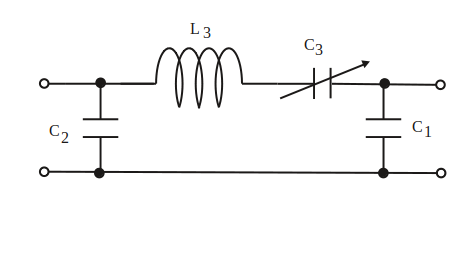
\includegraphics[width=3in]{figuras/osc11.png}\\
	\caption{Red de realimentación de un oscilador Clapp.}\label{osc11}
\end{figure}

En la figura \ref{osc12} a) se muestra un ejemplo práctico de un
oscilador Colpitts. Si se diseña para que: $\mid X_{C_L}\mid w_o$,
$\mid X_{C_E}\mid w_o$ y $\mid X_{C_B}\mid w_o$  $\rightarrow 0$ y
$\mid X_{L_{CRF}}\mid w_o \rightarrow \infty$, el circuito
equivalente de pequeña señal será el mostrado en la figura
\ref{osc12} b). Si se abre el lazo en la base de transistor y se
diseña para que el paralelo de $R_2$ con la resistencia de entrada
del transistor sea $\gg \mid X_{C_1}\mid w_o$, se pueden utilizar
las ecuaciones de diseño ya obtenidas : $w_o=\frac{\displaystyle
	1}{\displaystyle \sqrt{L_3C_1C_2/(C_1+C_2)}}$ y $g_m R_o>
\frac{\displaystyle C_1}{\displaystyle C_2}$. En este circuito la
frecuencia se puede ajustar con $L_3$ y la condición de amplitud con
la polarización mediante el ajuste de $R_E$.

Un ejemplo práctico de un oscilador Hartley es mostrado en la figura
\ref{osc13} a). Si se diseña para que: $\mid X_{C_E}\mid w_o$, $\mid
X_{C_o}\mid w_o$y $\mid X_{C_B}\mid w_o$ $\rightarrow 0$, el
circuito equivalente de pequeña señal será el mostrado en la figura
\ref{osc13} b). Si se abre el lazo en la base de transistor y se
diseña para que el paralelo de $R_2$ con la resistencia de entrada
del transistor sea $\gg \mid X_{L_1}\mid w_o$, se pueden utilizar
las ecuaciones de diseño ya obtenidas : $w_o=\frac{\displaystyle
	1}{\displaystyle \sqrt{C_3(L_1+L_2+2M)}}$ y $g_m R_o >
\frac{\displaystyle L_2+M}{\displaystyle L_1+M}$, siendo
$R_o=r_o\parallel R_{pL2}$, si $r_o$ es la resistencia de salida del
transistor y $R_{pL2}$ es la resistencia de pérdida de $L_2$. En
este circuito la frecuencia se puede ajustar con $C_3$ y la
condición de amplitud con la polarización mediante el ajuste de
$R_E$.


\begin{figure}
	\centering
	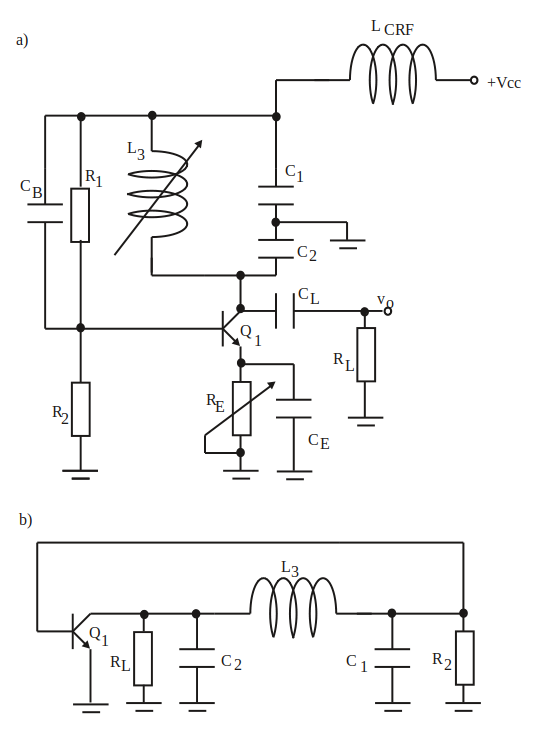
\includegraphics[width=3in]{figuras/osc12.png}\\
	\caption{Oscilador Colpìtts práctico: a) circuito, b) equivalente de pequeña señal.}\label{osc12}
\end{figure}

\begin{figure}
	\centering
	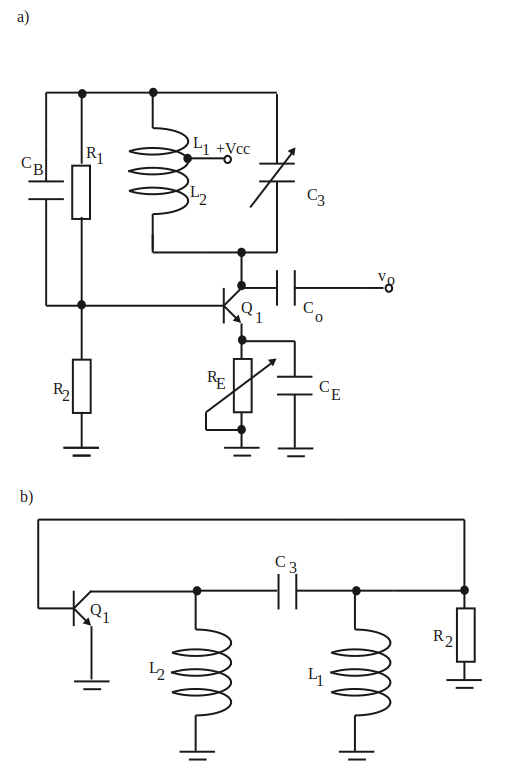
\includegraphics[width=3in]{figuras/osc13.png}\\
	\caption{Oscilador Hartley práctico: a) circuito, b) equivalente de pequeña señal.}\label{osc13}
\end{figure}

\subsection{Osciladores a cristal}

\hspace{10pt} Como se mencionó en el punto anterior, la estabilidad en frecuencia
de un oscilador tipo L-C depende directamente del factor de calidad
$Q$ del circuito sintonizado. En la práctica en este tipo de
circuitos, los valores máximos obtenibles de $Q$ están dentro del
orden de 200 a 300.

Cuando la estabilidad en frecuencia requerida es muy elevada, se
recurre a resonadores electromecánicos de elevada performance entre
los cuales se encuentran los cristales piezoeléctricos,
particularmente los de cuarzo. Estos cristales tienen la propiedad
de intercambiar energía eléctrica y mecánica; por ejemplo: una
fuerza aplicada en una dirección adecuada sobre el cristal,
originará la aparición de cargas eléctricas en su superficie. Por el
contrario, un potencial eléctrico aplicado causará un desplazamiento
mecánico en la superficie del material. La frecuencia de resonancia
electromagnética de estos cristales y el factor de calidad $Q$
dependen de: sus dimensiones físicas y tallado, la orientación
cristalina, del montaje del cristal sobre sus soportes mecánicos y
eléctricos. Hay cristales con frecuencias de resonancia desde unos
pocos Kilohertz hasta varios cientos de Megahertz, dependiendo de su
diseño y orientación. Los valores de $Q$ pueden ser diseñados desde
un rango de varios miles hasta varios cientos de miles. Estos
grandes valores de $Q$ y su excelente estabilidad con respecto al
tiempo y la temperatura los hacen ideales en el diseño de
osciladores donde la precisión y estabilidad en frecuencia son
asuntos críticos.

En la figura \ref{osc14} se muestra el símbolo circuital, el
circuito equivalente y las características de reactancia de un
cristal de cuarzo típico. El circuito equivalente de un cristal
puede ser descrito por un circuito RLC serie con un capacitor en
paralelo $C_p$, tal lo mostrado en la figura \ref{osc14} b).
Típicamente las reactancia asociadas a $L_s$ y $C_s$ son mucho
mayores que $R_s$, resultando por lo tanto un elevado valor de $Q$.

A modo de ejemplo un cristal de cuarzo de 90 KHz podría tener
valores típicos de: $L_s=137 H$, $C_s=0,0235 pF$ y $R_s= 15
k\Omega$, correspondiente a un $Q\approx 5160$. $C_p$ representa la
capacidad de los electrodos de contacto y su magnitud es típicamente
varios órdenes de magnitud mayor que $C_s$. En este ejemplo
$C_p\approx 4 pF$.

Si se desprecia el valor de $R_s$, la impedancia del cristal sería
una reactancia pura $jX$:

\begin{equation}\label{ecu24}
	Z_{cristal} = jX = \frac{\displaystyle -j}{\displaystyle wC_p}\left[\frac{\displaystyle
		w^2-w_s^2}{\displaystyle w^2-w_p^2
	}\right]
\end{equation}

, dónde

\begin{equation}\label{ecu24}
	w_s = 2\pi f_s= \left[\frac{\displaystyle
		1}{\displaystyle L_sC_s
	}\right]^{1/2}
\end{equation}

y

\begin{equation}\label{ecu24}
	w_p = 2\pi f_p= \left[\frac{\displaystyle 1}{\displaystyle L_s}\left(\frac{\displaystyle
		1}{\displaystyle C_s}+\frac{\displaystyle
		1}{\displaystyle C_p}\right)\right]^{1/2}
\end{equation}

La frecuencia de resonancia serie (impedancia cero) es $w_s$ y la
paralelo (impedancia infinita) es $w_p$. Es de notar que $w_p$ es
siempre mayor que $w_s$. En la mayor parte de los cristales $C_p\gg
C_s$, por lo que $w_p\approx w_s$. Como ejemplo en el cristal de
$90KHz$ ya mencionado $w_p$ es sólo $0,3\%$ mayor que $w_s$,
pudiendo reducirse más aún la diferencia si se agrega capacidad en
paralelo.

La figura \ref{osc14} c) muestra cualitativamente la curva de la
reactancia de un cristal en la vecindad de sus frecuencias
resonantes. En el estrecho rango en el cual $w_s<w<w_p$, el cristal
se comporta inductivamente, fuera de ese rango se comporta
capacitivamente. El cristal se utiliza principalmente en su región
inductiva, es decir en el rango de frecuencias entre $w_s$ y $w_p$.
Dado que ambas frecuencias de resonancia son muy cercanas la
frecuencia del oscilador resultante es precisa y estable,
determinada sólo por las características del cristal, el rol del
resto del circuito es proveer la ganancia suficiente para asegurar
que la ganancia de lazo sea $\geq 1$ para oscilaciones sostenidas.

\begin{figure}
	\centering
	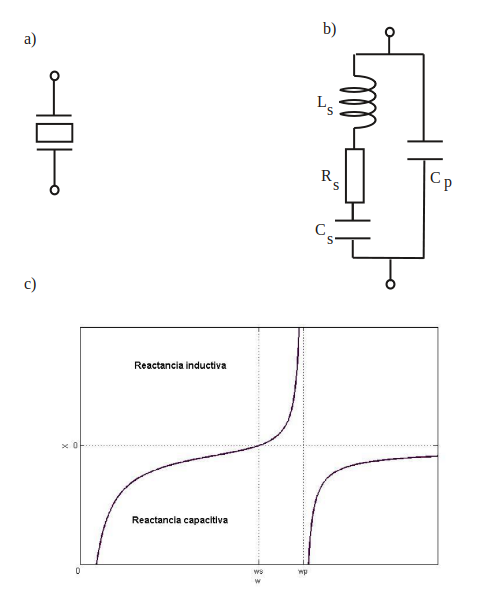
\includegraphics[width=5in]{figuras/osc14.png}\\
	\caption{Cristal de cuarzo: a) símbolo circuital, b) circuito equivalente y c) característica de reactancia suponiendo despreciable $R_s$.}\label{osc14}
\end{figure}


Las configuraciones de osciladores a cristal más utilizadas son las
mostradas esquemáticamente en la figura \ref{osc15}. El caso a) es
un oscilador tipo Colpitts en el cual el inductor $L_3$ (figura
\ref{osc10} a)) es reemplazado por el cristal, éste funcionará en su
zona inductiva y el circuito oscilará a una frecuencia intermedia
entre $w_s$ y $w_p$ si se cumple adecuadamente la condición de
amplitud, este oscilador se denomina Pierce. El caso de la figura
\ref{osc15} b) es un oscilador sin desplazamiento de fase, por lo
tanto la condición de fase sólo se cumple a la frecuencia de
resonancia serie $w_s$, es decir que este circuito oscilará a dicha
frecuencia si se cumple la condición de amplitud.

Las figuras \ref{osc16} a) y b) muestran posibles configuraciones
prácticas de osciladores a cristal. El caso a) es un oscilador sin
desplazamiento de fase, la frecuencia de oscilación será $w_s$,
mientras que la condición de amplitud se cumplirá si la ganancia de
lazo es $\geq1$ a $w_s$, ésta se calcula reemplazando el cristal por
su resistencia serie $R_s$. El oscilador de la figura \ref{osc16} b)
responde a la configuración Pierce y utiliza un inversor CMOS como
amplificador inversor de gran ganancia, el cristal trabaja en su
zona inductiva y la frecuencia de oscilación será $w_s<w_{osc}<w_p$,
debido a que $w_s$ y $w_p$ son muy cercanas la frecuencia de
oscilación está determinas con un importante grado de precisión.

\begin{figure}
	\centering
	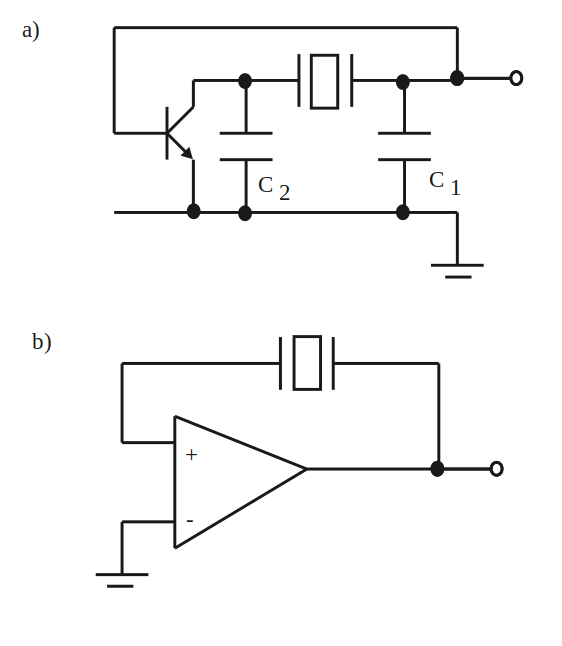
\includegraphics[width=2.5in]{figuras/osc15.png}\\
	\caption{Configuraciones básicas de osciladores a cristal: a) tipo Pierce, b) sin desplazamiento de fase.}\label{osc15}
\end{figure}

\begin{figure}
	\centering
	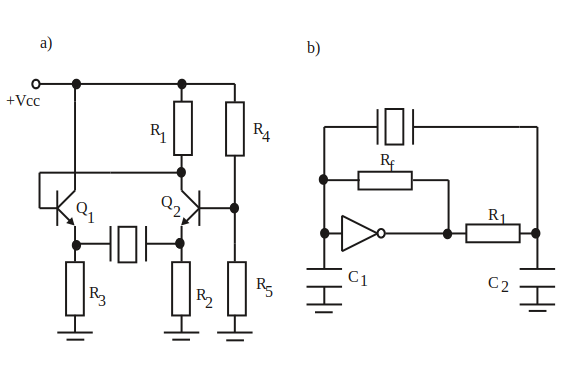
\includegraphics[width=3.5in]{figuras/osc16.png}\\
	\caption{Configuraciones prácticas de osciladores a cristal: a) sin desplazamiento de fase, b) tipo Pierce con inversor CMOS.}\label{osc16}
\end{figure}
